\begin{figure}[b]
\centering 
\subfloat[Notch joints.] {
  \label{fig:joint-notch} 
  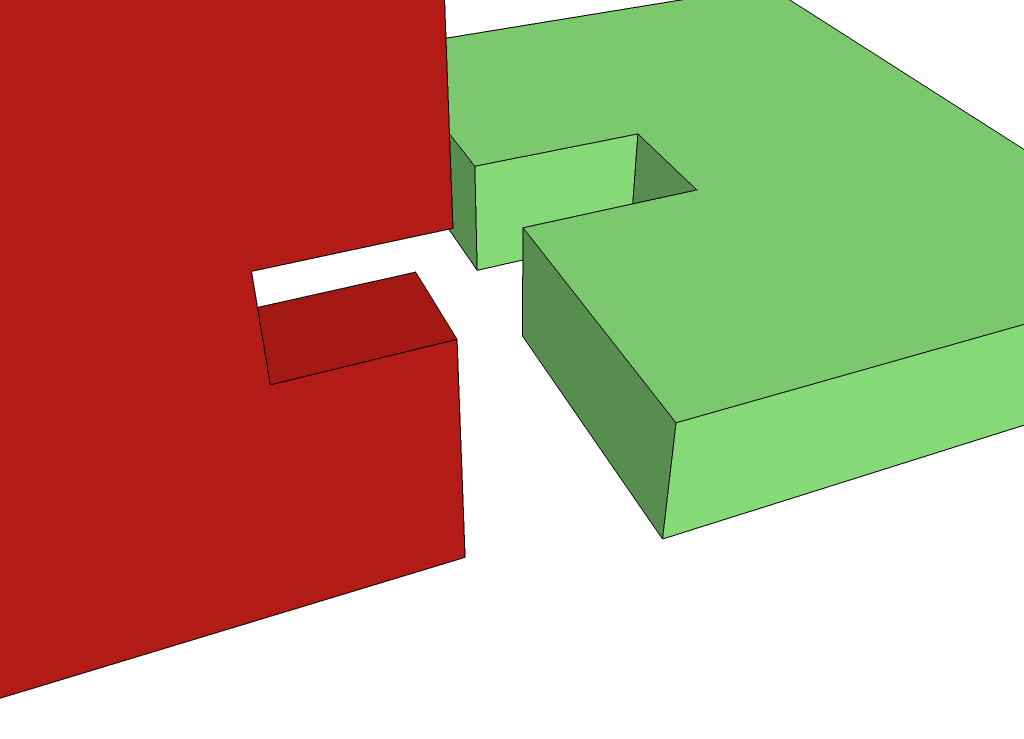
\includegraphics[width=0.3\linewidth]{img/joint-notch.png}
}
\subfloat[Finger (box) joints.] {
    \label{fig:joint-finger}
    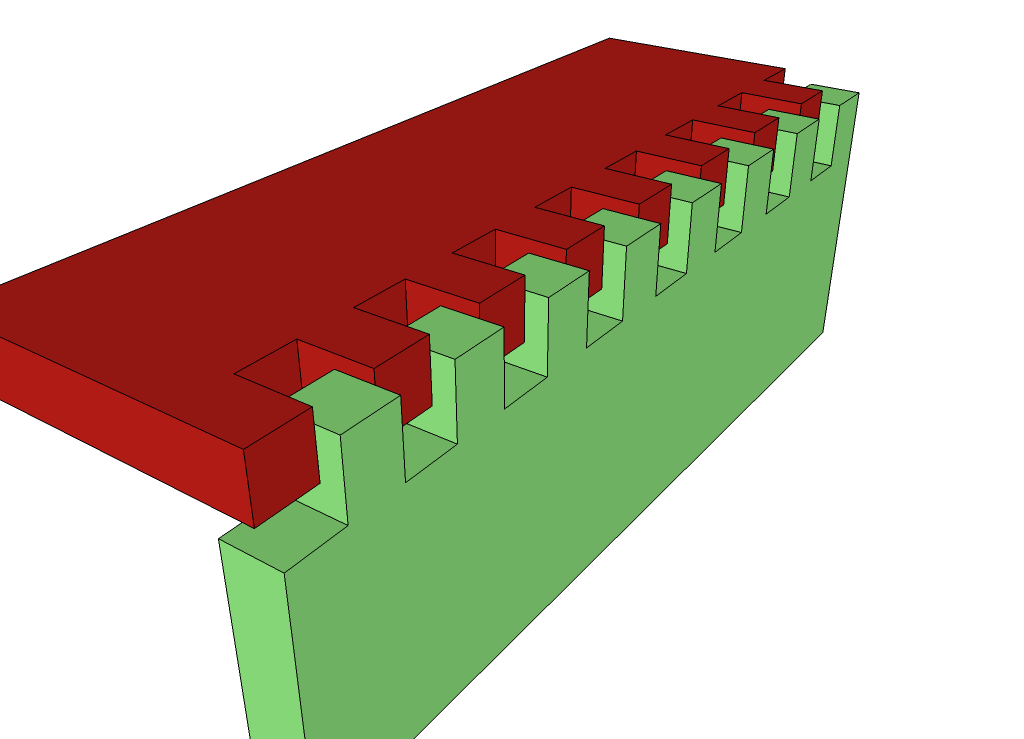
\includegraphics[width=0.3\linewidth]{img/joint-finger.png}
}
\caption[Two common notch types]{Two common methods to join
  parts. Notch joints are used when parts intersect along part
  midsections; finger joints (box joints) join parts along edges.}
\label{fig:joint}
\end{figure}
